\chapter{Desenvolvimento}
Neste capítulo são apresentados a metodologia e detalhes sobre o desenvolvimento do trabalho.
Nos itens deste capítulo será apresentada a metodologia e detalhado o desenvolvimento do software da biblioteca,
demonstrando requisitos, arquitetura, ambiente de implementação, documentação e implementação.


\section{Metodologia}
Esta seção descreve a metodologia proposta para o desenvolvimento da biblioteca a ser produzida por este trabalho,
levando em consideração as peculiaridades do trabalho e os objetivos específicos a serem alcançados.

A biblioteca será desenvolvido utilizando uma abordagem iterativa incremental, conforme descrito por \cite{met}
incrementada com as características de metodologia vistas como necessárias para o desenvolvimento de uma biblioteca em
Python.
Esta metodologia permite refinamentos contínuos e adições incrementais de funcionalidades, garantindo que o software
evolua de forma eficaz ao longo do projeto, além de prever etapas de estudo e estruturação, essenciais para esse
tipo de de projeto.
As etapas incluem:

\begin{itemize}
    \item Escolha do escopo do projeto: Alinhamento e definição do que será implementado;
    \item Estudo dos conceitos e ferramentas: Estudo de conceitos e ferramentas que serão utilizados durante o projeto;
    \item Estudo dos casos de uso: Estudo e criação dos casos de uso para compreensão dos requisitos funcionais gerais;
    \item Prototipagem Rápida: Criação de versões iniciais para testar conceitos básicos;
    \item Projeto da Estrutura: Desenvolvimento dos diagramas de classe para estruturar a implementação;
    \item Desenvolvimento Iterativo: Melhoria contínua do software através de ciclos repetidos de desenvolvimento e teste;
    \item Documentação: Desenvolvimento da documentação da biblioteca;
    \item Expansão Incremental: Adição gradual de novas funcionalidades, alinhadas com os requisitos do projeto.
\end{itemize}

Reuniões periódicas com a orientadora foram realizadas para acompanhamento, esclarecimento de dúvidas e ajustes
necessários.

\section{Requisitos da Biblioteca}

Com base nos objetivos específicos propostos na introdução do trabalho, foi realizado o estudo dos casos de uso da
biblioteca, levantando requisitos de forma mais detalhada e concebendo uma visão inicial das dinâmicas de uso e
funcionamento da biblioteca.
Isso foi realizado tendo como base a uma sequencia de ações prováveis que um usuário faria durante o uso da ferramenta.

O resultado da análise foi o seguinte diagrama de casos de uso, que denota um caminho provável de ações do usuário:

\begin{figure}[H]
    \centering
    \caption{Casos de uso}
    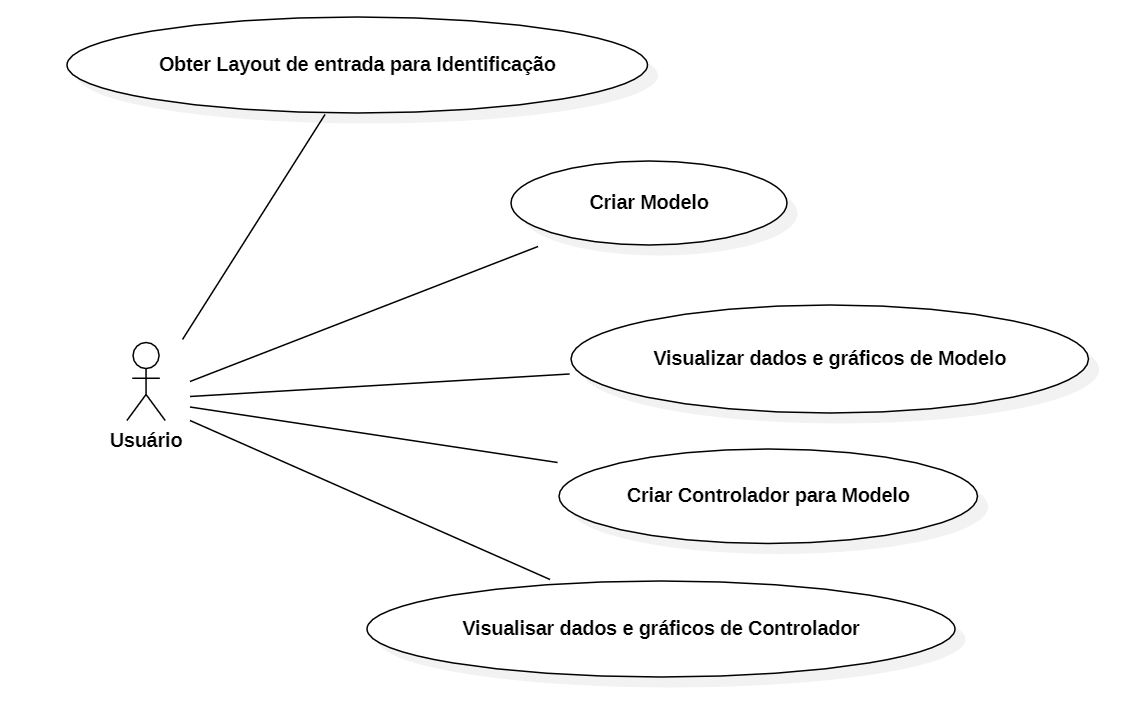
\includegraphics[scale=0.5]{figuras/use_cases}
    \label{fig:use_cases}
    \\
    \vspace{0cm}\hspace{0cm}\small{Fonte: Do autor}
\end{figure}

As tabelas \ref{tab:uc1}, \ref{tab:uc2}, \ref{tab:uc3}, \ref{tab:uc4}, \ref{tab:uc5} detalham os casos de uso ilustrado
na figura \ref{fig:use_cases}, especificando o objetivo, os pré requisitos e o cenário de cada caso de uso.


\begin{table}[H]
    \begin{center}
        \begin{tabularx}{\textwidth}{|>{\bfseries\raggedright\arraybackslash\center}m{5cm}|X|}
            \hline
            Identificador UC: UC-1\newline Diagrama ID: D-1 & Nome: Obtenção de layout de input de dados para identificação\newline Prioridade: Alta                                                                                                                                                                                                   \\ \hline
            Objetivo                                        & Fornecer planilha de layout para que sejam inseridos os dados necessários para um determinado processo de identificação.                                                                                                                                                                 \\ \hline
            Atores                                          & Usuário                                                                                                                                                                                                                                                                                  \\ \hline
            Restrições                                      & Deve-se salvar a planilha referente ao layout necessário.                                                                                                                                                                                                                                \\ \hline
            Pré-condições                                   & -                                                                                                                                                                                                                                                                                        \\ \hline
            Cenário principal                               & 1. O método é chamado, recebendo o caminho onde deve salvar o arquivo e possívelmente os parâmetros referentes ao layout em espessífico, como tipo de arquivo, por exemplo.\newline 2. É construido em memória o layout desejado.\newline 3. É salvo o arquivo no caminho espessificado. \\ \hline
            Pós condições                                   & O Usuário possui o layout e pode inserir os dados.                                                                                                                                                                                                                                       \\ \hline
        \end{tabularx}
        \caption{Obtenção de layout de input de dados para identificação}
        \label{tab:uc1}
    \end{center}
\end{table}

\begin{table}[H]
    \begin{center}
        \begin{tabularx}{\textwidth}{|>{\bfseries\raggedright\arraybackslash\center}m{5cm}|X|}
            \hline
            Identificador UC: UC-2\newline Diagrama ID: D-2 & Nome: Identificação de sistema\newline Prioridade: Alta                                                                                                                                                                                                                                             \\ \hline
            Objetivo                                        & Realizar processo de identificação do sistema baseado nos dados e obter modelo.                                                                                                                                                                                                                      \\ \hline
            Atores                                          & Usuário                                                                                                                                                                                                                                                                                              \\ \hline
            Restrições                                      & Deve-se obter o modelo do sistema.                                                                                                                                                                                                                                                                   \\ \hline
            Pré-condições                                   & layout de dados preenchido.                                                                                                                                                                                                                                                                          \\ \hline
            Cenário principal                               & 1. O método de identificação é chamado, recebendo o caminho do arquivo de layout e possívelmente os parâmetros referentes ao método em espessífico.\newline 2. São realizados os cálculos e é obtido o objeto de modelo do sistema.\newline 3. O objeto de modelo do sistema é retornado ao usuário. \\ \hline
            Pós condições                                   & O Usuário possui um objeto de modelo do sistema.                                                                                                                                                                                                                                                     \\ \hline
        \end{tabularx}
        \caption{Identificação de sistema}
        \label{tab:uc2}
    \end{center}
\end{table}

\begin{table}[H]
    \begin{center}
        \begin{tabularx}{\textwidth}{|>{\bfseries\raggedright\arraybackslash\center}m{5cm}|X|}
            \hline
            Identificador UC: UC-3\newline Diagrama ID: D-3 & Nome: Visualização de modelo de sistema\newline Prioridade: Alta                                                                                                                                                                                                                         \\ \hline
            Objetivo                                        & Visualizar gráfico e dados indicadores importantes de um modelo.                                                                                                                                                                                                                         \\ \hline
            Atores                                          & Usuário                                                                                                                                                                                                                                                                                  \\ \hline
            Restrições                                      & Deve ser possível visualisar gráfico e dados indicadores importantes do modelo.                                                                                                                                                                                                          \\ \hline
            Pré-condições                                   & O Usuário possui um objeto de modelo do sistema.                                                                                                                                                                                                                                         \\ \hline
            Cenário principal                               & 1. Um método de visualisação de dados ou gráfico é chamado, passando possíveis parâmetros necessários ou que irão mudar a forma como os dados serão exibidos.\newline 2. São preparados os objetos a serem exibidos ao usuário.\newline 3. São exibidos os dados ou gráficos ao usuário. \\ \hline
            Pós condições                                   & O Usuário pode visualisar os dados do modelo.                                                                                                                                                                                                                                            \\ \hline
        \end{tabularx}
        \caption{Visualização de modelo de sistema}
        \label{tab:uc3}
    \end{center}
\end{table}

\begin{table}[H]
    \begin{center}
        \begin{tabularx}{\textwidth}{|>{\bfseries\raggedright\arraybackslash\center}m{5cm}|X|}
            \hline
            Identificador UC: UC-4\newline Diagrama ID: D-4 & Nome: Aproximação de Controlador baseado em modelo de sistema\newline Prioridade: Alta                                                                                                                                                                                                     \\ \hline
            Objetivo                                        & Obter aproximação de parâmetros de controle baseados no modelo obtido.                                                                                                                                                                                                                     \\ \hline
            Atores                                          & Usuário                                                                                                                                                                                                                                                                                    \\ \hline
            Restrições                                      & Deve-se obter uma aproximação dos parâmetros do controlador.                                                                                                                                                                                                                               \\ \hline
            Pré-condições                                   & O Usuário possui um objeto de modelo do sistema.                                                                                                                                                                                                                                           \\ \hline
            Cenário principal                               & 1. O método de aproximação é chamado, recebendo o modelo do sistema e possívelmente os parâmetros referentes ao método de aproximação em espessífico.\newline 2. São realizados os cálculos e é obtido o objeto de controlador.\newline 3. O objeto de controlador é retornado ao usuário. \\ \hline
            Pós condições                                   & O Usuário possui um objeto de controlador.                                                                                                                                                                                                                                                 \\ \hline
        \end{tabularx}
        \caption{Aproximação de Controlador baseado em modelo de sistema}
        \label{tab:uc4}
    \end{center}
\end{table}

\begin{table}[H]
    \begin{center}
        \begin{tabularx}{\textwidth}{|>{\bfseries\raggedright\arraybackslash\center}m{5cm}|X|}
            \hline
            Identificador UC: UC-5\newline Diagrama ID: D-5 & Nome: Visualização de controlador\newline Prioridade: Alta                                                                                                                                                                                                                               \\ \hline
            Objetivo                                        & Visualizar gráfico e dados indicadores importantes de um controlador.                                                                                                                                                                                                                    \\ \hline
            Atores                                          & Usuário                                                                                                                                                                                                                                                                                  \\ \hline
            Restrições                                      & Deve ser possível visualisar gráfico e dados indicadores importantes do controlador gerado.                                                                                                                                                                                              \\ \hline
            Pré-condições                                   & O Usuário possui um objeto de controlador.                                                                                                                                                                                                                                               \\ \hline
            Cenário principal                               & 1. Um método de visualisação de dados ou gráfico é chamado, passando possíveis parâmetros necessários ou que irão mudar a forma como os dados serão exibidos.\newline 2. São preparados os objetos a serem exibidos ao usuário.\newline 3. São exibidos os dados ou gráficos ao usuário. \\ \hline
            Pós condições                                   & O Usuário pode visualisar os dados do controlador.                                                                                                                                                                                                                                       \\ \hline
        \end{tabularx}
        \caption{Visualização de controlador}
        \label{tab:uc5}
    \end{center}
\end{table}




\section{Descrição da arquitetura}\label{sec:descarc}

A fim de construir uma biblioteca com arquitetura de código compreensível e escalável, optou-se pela orientação
da mesma a classes e objetos, visto que este tipo de abordagem resulta em uma estrutura clara e amplamente utilizada.
Baseado nisso e nos casos de uso, foi desenvolvido o diagrama de classes da figura \ref{fig:class_diag}, que caracteriza
as classes da biblioteca, detalhando seus atributos e métodos, além de apontar os relacionamentos e dependências entre
as classes.

\begin{figure}[H]
    \centering
    \caption{Diagrama de classes}
    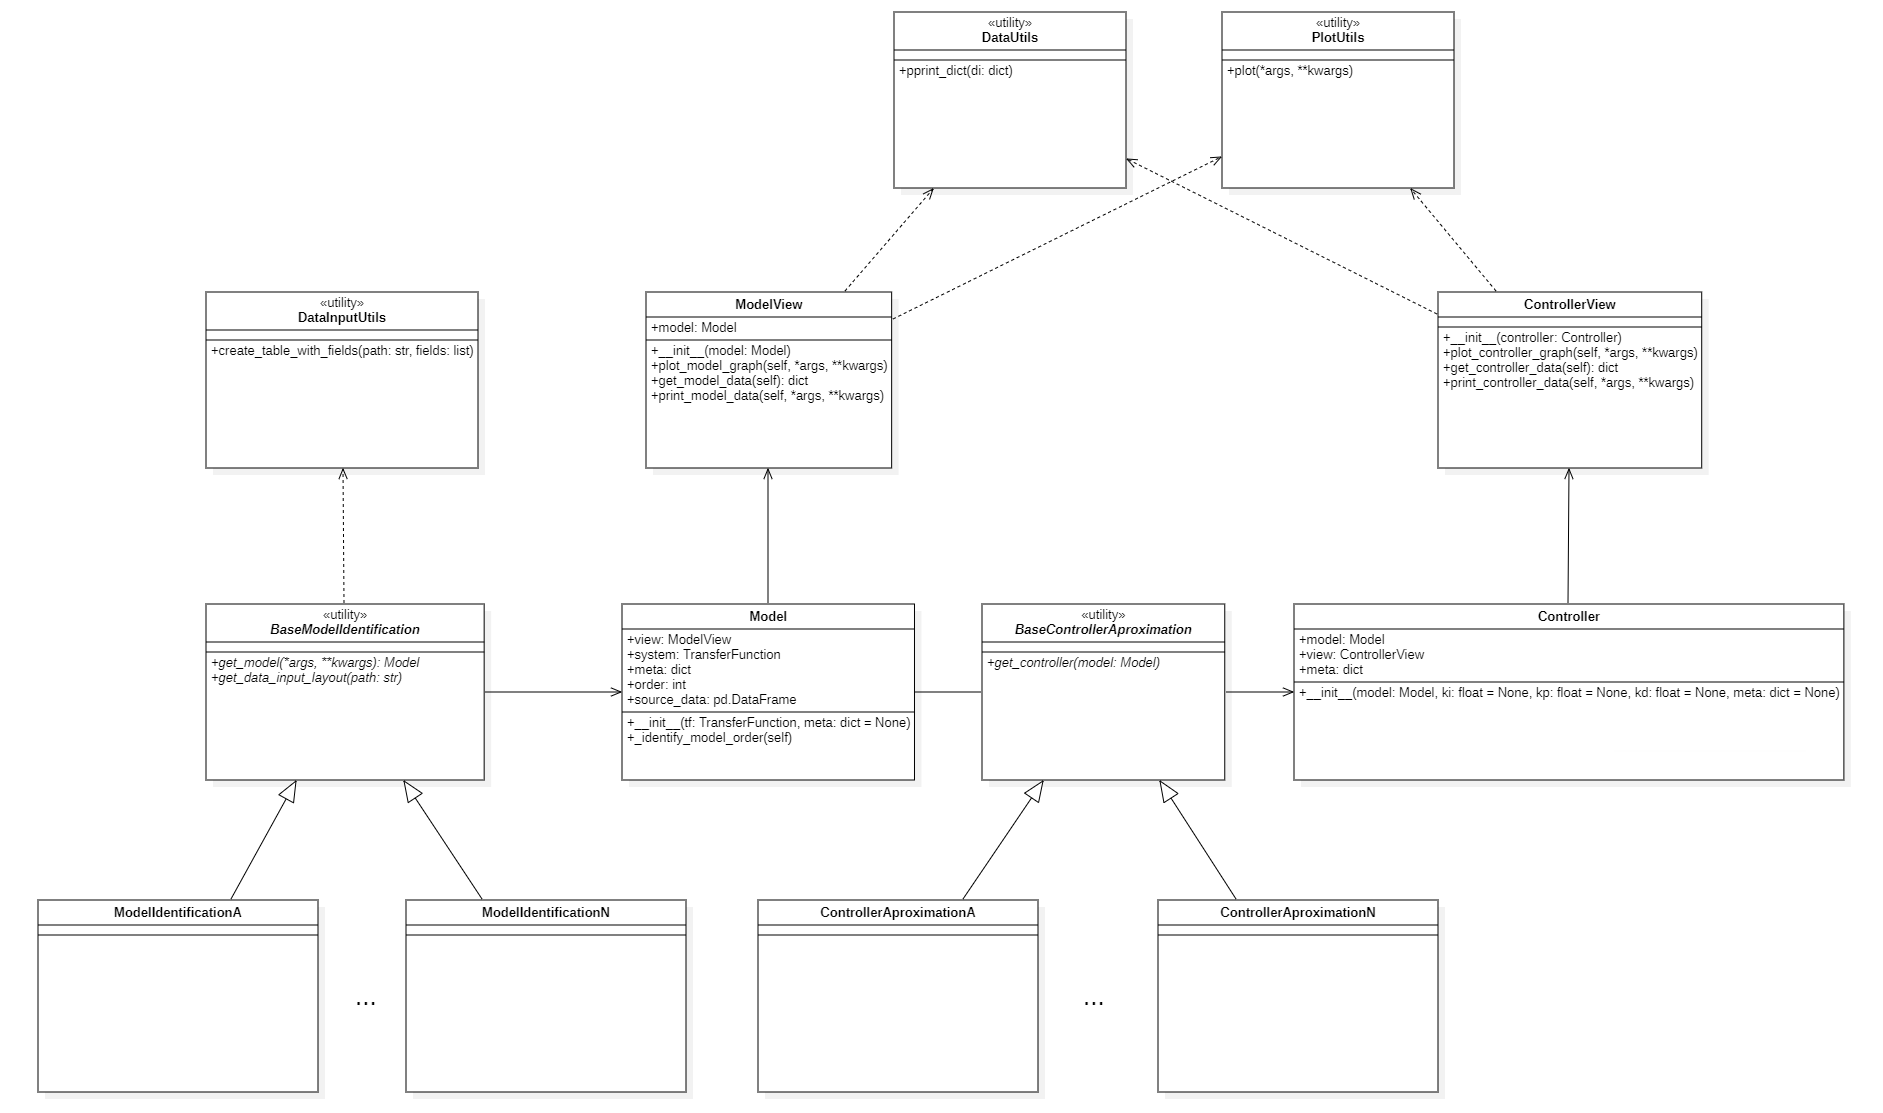
\includegraphics[scale=0.32]{figuras/class_diag}
    \label{fig:class_diag}
    \\
    \vspace{0cm}\hspace{0cm}\small{Fonte: Do autor}
\end{figure}

Tendo em vista que o diagrama da figura \ref{fig:class_diag} é grande demais para ser discutido em apenas uma figura,
as subseções desta sessão tratam das classes específicas presentes no diagrama, com visões ampliadas das mesmas para
facilitar a visualização.

\subsection{DataInputUtils}

Classe utilitária, ou seja, não deve ser instanciada como objeto, para a entrada de dados externos.
É previsto nela o método create\_table\_with\_fields cujo intuito é a criação de uma tabela com campos espessíficos,
conforme requisitado pelo caso de uso descrito na tabela \ref{tab:uc1}.
A visão ampliada da classe no diagrama pode ser melhor observada na figura \ref{fig:class_diag_diubmi};

\begin{figure}[H]
    \centering
    \caption{Diagrama de classes ampliado - DataInputUtils e BaseModelIdentification}
    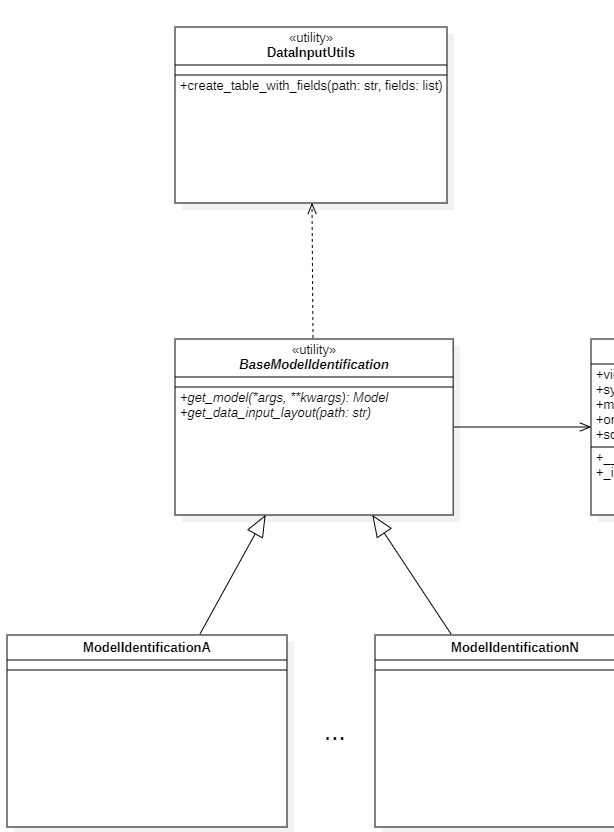
\includegraphics[scale=0.6]{figuras/class_diag_diubmi}
    \label{fig:class_diag_diubmi}
    \\
    \vspace{0cm}\hspace{0cm}\small{Fonte: Do autor}
\end{figure}

\subsection{DataUtils}

Esta é outra classe utilitária, similar a DataInputUtils, mas com o foco na manipulação de dados em memória.
Seu objetivo é fornecer e centralizar ferramentas de manipulação de dados que serão utilizadas em toda a biblioteca.
A classe, e seus relacionamentos inicialmente idealizados, pode ser vista na figura \ref{fig:class_diag_dupu}.
Os métodos dessa classe foram criados de acordo com as necessidades encontradas durante o desenvolvimento, de forma que
neste diagrama inicial consta apenas o método pprint\_dict, criado a caráter de exemplo, que mais tarde foi reenquadrado
para a classe PlotUtils.

\begin{figure}[H]
    \centering
    \caption{Diagrama de classes ampliado - DataUtils e PlotUtils}
    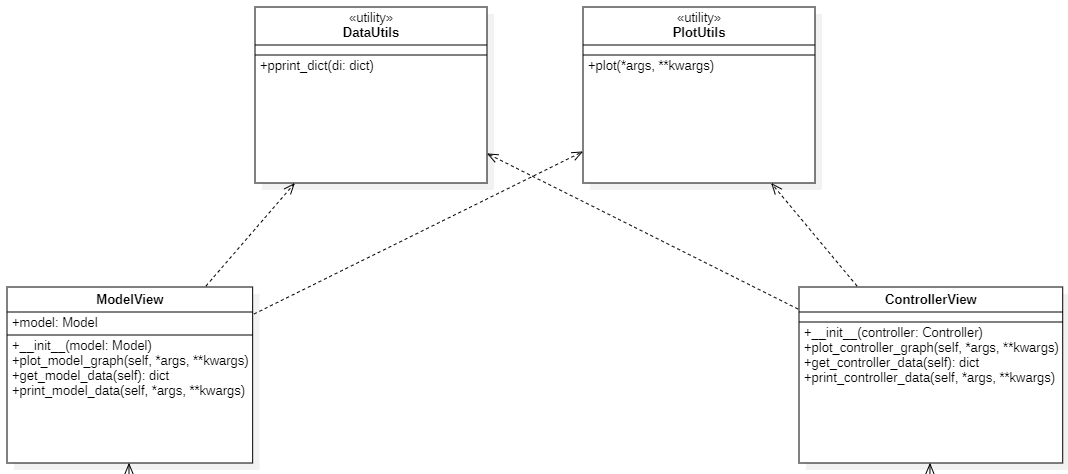
\includegraphics[scale=0.6]{figuras/class_diag_dupu}
    \label{fig:class_diag_dupu}
    \\
    \vspace{0cm}\hspace{0cm}\small{Fonte: Do autor}
\end{figure}

\subsection{PlotUtils}

PlotUtils é mais uma classe utilitária, seu objetivo é fornecer e centralizar ferramentas de visualização de dados
a serem utilizadas pelas classes ModelView e ControllerView, como apresentado na figura \ref{fig:class_diag_dupu}.
Em sua lista de métodos é definido plot, uma ferramenta crucial para viabilizar os requerimentos dos usos de caso
\ref{tab:uc3} e \ref{tab:uc5}, visto que seu objetivo é a impressão dos gráficos de resposta a sinal degrau de funções de
transferência.
De forma similar a classe DataUtils, também foram criados outros métodos para esta classe de acordo com as necessidades de
desenvolvimento.

\subsection{Model}

Classe representativa do Modelo matemático de uma planta de sistemas de controle, apresentada na figura
\ref{fig:class_diag_model}, foi projetada para guardar atributos
referentes a função de transferência e ordem do modelo, além dos dados discretos utilizados para obtenção do modelo,
caso existam, um dicionário para metadados (mais tarde removido), e view, um objeto da classe ModelView, para
possibilita o acesso as funcionalidades de visualização de dados a partir do objeto de modelo.
Também são descritos no diagrama os métodos de inicialização, que recebe alguns dos atributos da classe, e um método
interno para obtenção da ordem da função de transferência do modelo.

\begin{figure}[H]
    \centering
    \caption{Diagrama de classes ampliado - Model e ModelView}
    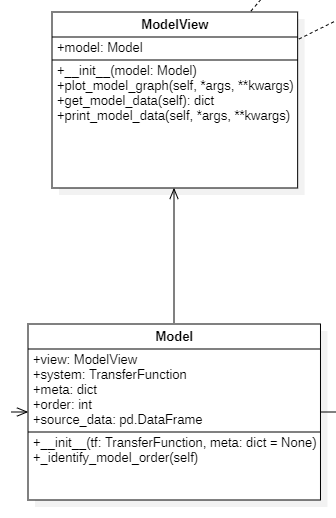
\includegraphics[scale=0.7]{figuras/class_diag_model}
    \label{fig:class_diag_model}
    \\
    \vspace{0cm}\hspace{0cm}\small{Fonte: Do autor}
\end{figure}

\subsection{ModelView}

A classe ModelView foi concebida como um meio termo entre a classe de modelo, Model, cujo foco é guardar os dados
referentes a um modelo, e não necessariamente apresenta-los ao usuário, e a classe PlotUtils, que fornece ferramentas
de visualização de dados gerais, que precisam de configurações espessíficas para apresentar os dados de modelo
corretamente.
Desta forma isolando as responsabilidades de cada componente.
Na figura \ref{fig:class_diag_model} é possível visualizar a classe, bem como seu atributo model recebido em sua
instanciação e seus métodos de instanciação (\_\_init\_\_), plot\_model\_graph, utilizado para apresentação de dados de
resposta do modelo a sinal degrau e comparação do modelo com so dados discretos utilizados para obte-lo,
get\_model\_data, que retorna dados de resposta a sinal degram do modelo, como sobressinal e tempo de acomodação, e
print\_model\_data que apresenta os dados de get\_model\_data ao usuário de forma formatada.

\subsection{BaseModelIdentification}

Na figura \ref{fig:class_diag_diubmi}, é apresentada a classe utilitária e abstrata BaseModelIdentification, seu
propósito é padronizar os métodos de identificação de modelo, de forma que todos eles sejam subclasses dela.
Assim sendo, o método abstrato get\_model, que calcula e retorna um objeto de modelo (Model), deve ser implementado em
todas as suas subclasses obrigatoriamente.
Além disso também é previsto o método get\_data\_input para fornecer ao usuário o modelo de tabela a ser preenchido
com os dados para identificação.

Ainda na figura \ref{fig:class_diag_diubmi} são denotadas as classes ModelItentificationA e ModelItentificationN de
forma ilustrativa, representando subclasses que criadas durante o desenvolvimento da biblioteca.

\begin{figure}[H]
    \centering
    \caption{Diagrama de classes ampliado - Controller e ControllerView}
    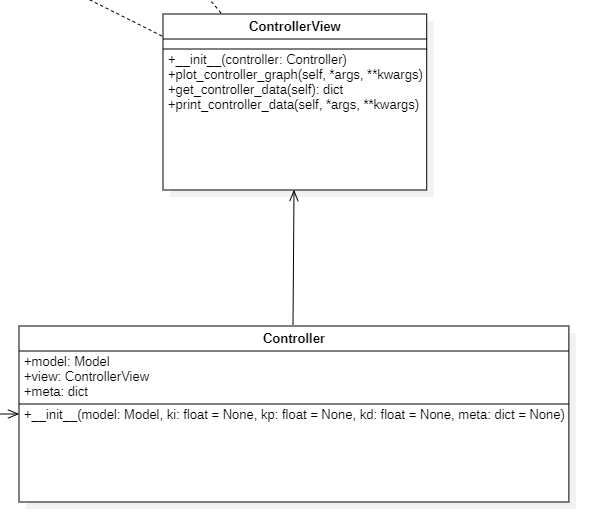
\includegraphics[scale=0.7]{figuras/class_diag_controller}
    \label{fig:class_diag_controller}
    \\
    \vspace{0cm}\hspace{0cm}\small{Fonte: Do autor}
\end{figure}

\subsection{Controller}

Controller é bastante similar a Model, no quesito de que sua finalidade é salvar os dados de uma função de
transferência, bem como dados acessórios a mesma, além de possibilitar sua visualização pelo atributo view, uma
instância de ControllerView em vez de ModelView.
Em sua instanciação, recebe um objeto de modelo e os ganhos PID a serem considerados para o controlador, que, ainda no
momento da instanciação, serão utilizados para o fechamento da malha, sendo a função de transferência salva referente
ao modelo da planta em malha fechada.
A classe pode ser melhor visualizada na figura \ref{fig:class_diag_controller};

\subsection{ControllerView}

ControllerView implementa métodos identicos a ModelView, mas com o foco no objeto controller, e com a diferença de que
o método plot\_model\_graph entende por padrão mostrar a comparação entre a resposta a sinal degrau do modelo em malha
aberta e o modelo em malha fechada com o controlador, ao invés da comparação com os dados discretos.
Pode ser visualizada na figura \ref{fig:class_diag_controller};

\subsection{BaseControllerAproximation}

Classe idêntica a BaseModelIdentification mas com o foco em obter um objeto da classe Controller.
Ao invés de get\_model, implementa o método abstrato get\_controller.
A classe e as visões ilustrativas de suas subclasses podem ser observadas na figura \ref{fig:class_diag_bcacontroller}.

\begin{figure}[H]
    \centering
    \caption{Diagrama de classes ampliado - BaseControllerAproximation}
    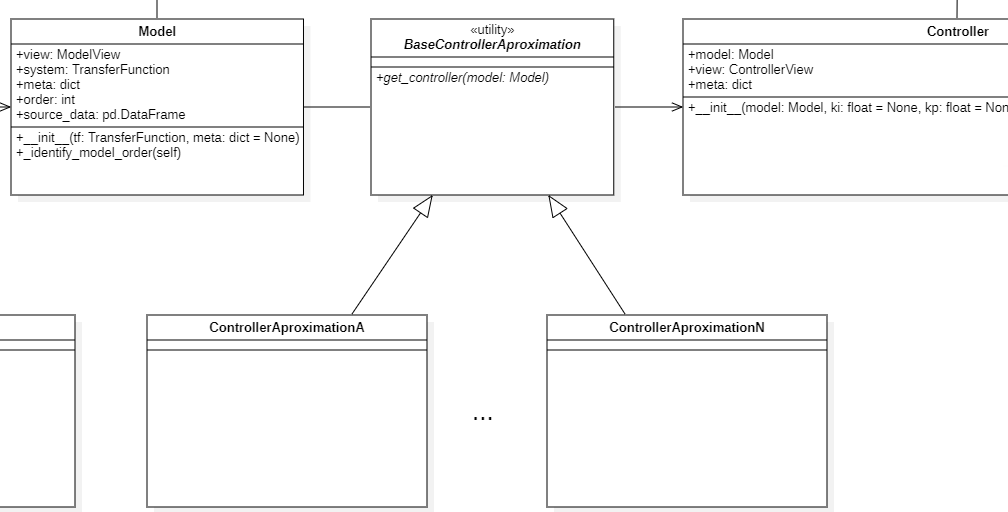
\includegraphics[scale=0.6]{figuras/class_diag_bcacontroller}
    \label{fig:class_diag_bcacontroller}
    \\
    \vspace{0cm}\hspace{0cm}\small{Fonte: Do autor}
\end{figure}


\section{Descrição do ambiente de implementação}

Nesta sessão serão explorados itens referentes ao ambiente de implementação utilizado para o
desenvolvimento, todos visando necessidades para implementação e publicação da biblioteca ou boas práticas de
desenvolvimento.

Para possibilitar a manutenção do código e facilitar futuras implementações é necessária a adoção de uma
estrutura de código e pastas que seja comum a comunidade, além disso existe a necessidade de uma estrutura compatível
com a publicação do código da biblioteca e do isolamento do código fonte da biblioteca dos testes da mesma.
Com isso em mente, foi adotada a estrutura apresentada em \cite{auto_test_vid}, que atende a essas necessidades.

\subsection{Controle de versão}

Foi escolhido o Git como opção de sistema de controle de versões da biblioteca.
Ele é um sistema de controle de versões preferido da comunidade, devido a sua alta performance, natureza decentralizada
e funcionalidades robustas para manipulação de grandes projetos \cite{usegit}.
Além de ser gratuito e de código aberto, é amplamente utilizado e integrado em um pletora de ferramentas e repositórios
como GitHub.

\subsection{Verificações e Testes}
\begin{figure}
    \centering
    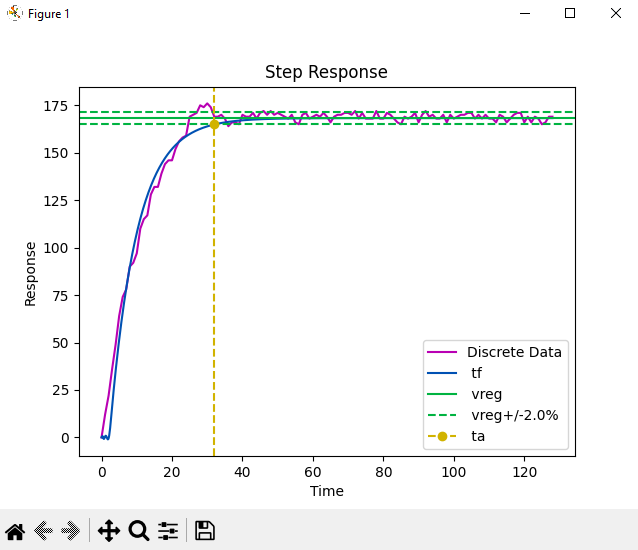
\includegraphics{C:\Users\luiz\PycharmProjects\tcc\figuras\get_model_plot}
    \caption{}
    \label{fig:}
\end{figure}
Nesta sessão será abordado o uso de ferramentas de verificação de código como Mypy e Flake8, bem como ferramentas
que foram utilizadas para automação de testes, como Pytest, tox e GitHub actions.

\subsubsection{Mypy e Flake8}
Ambas as ferramentas Mypy e Flake8 foram utilizadas durante o desenvolvimento para verificar erros de tipagem e
adequação ao PEP 8, de forma que o resultado final passa nas verificações de ambas as ferramentas.
Elas também foram adicionadas ao processo de automação de testes descrito em \ref{subsubsec:devtox}, para que não
ficassem apenas a cardo do uso manual pelo desenvolvedor.

\subsubsection{Pytest}

Para cada uma das classes implementadas foram desenvolvidos testes unitários, para validação de suas funcionalidades e
garantia de que implementações futuras que alterem os resultados de funcionalidades já implementadas, possivelmente de
forma incorreta, não passem despercebidas gerando falhas ao rodar os testes.

\subsubsection{tox}\label{subsubsec:devtox}

A ferramenta tox foi utilizada para automatizar a execução das verificações, com Mypy e Flake8, e testes unitários, com
PyTest, para as versões 3.9 e 3.10 do Python.
De forma que ao roda-lo, com base no arquivo de configuração criado, são instaladas as dependências do projeto em um
ambiente virtual e são executadas todas as verificações e testes.

\subsubsection{GitHub Actions}

Foi utilizada a plataforma de CI/CD do GitHub, GitHub Actions para a criação de um workflow de testes, que roda a
ferramenta tox descrita em \ref{subsubsec:devtox}, em ambientes Windows e Linux, toda vez que um pull é feito em uma
branch ou que é realizado um merge request.
Desta forma é automatizado o processo de testagem em diversos ambientes, que pode ser mais demorado e atrapalhar o
fluxo de desenvolvimento.
Além de garantir que os testes sejam sempre rodados para toda alteração que for feita no repositório.

\subsection{Documentação do código}

A documentação de código foi desenvolvida juntamente as implementações de cada classe.
Optou-se pelo uso da ferramenta Sphinx para a documentação de código utilizando o tema do projeto Read the Docs, onde
também foi hospedada como um projeto de código aberto e seguindo uma estrutura de documentação similar a da
biblioteca Python Control Systems Library.

\subsubsection{Sphinx}

Para a documentação em Sphinx foram desenvolvidas diversas páginas em \textit{reStructuredText} tratando dos seguintes itens:
\begin{alineas}
    \item \textbf{index}: Página principal da documentação com breve introdução e sumário da documentação;
    \item \textbf{Sobre}: Visão geral do projeto e guia de instalação;
    \item \textbf{Introdução}: Início rápido com exemplos e explicações práticas, e explicação geral do funcionamento da biblioteca;
    \item \textbf{Referência de Classes}: Listagem de todas as classes implementadas com breve resumo para cada grupo de classes;
    \item \textbf{Referências}: Página de glossário e referências bibliográficas utilizadas na documentação;
    \item \textbf{Desenvolvimento}: Página com orientações ao desenvolvimento.
\end{alineas}

Além disso a documentação de todas as classes e métodos implementados foi feita juntamente ao código fonte, através de
\textit{docstrings} suportadas que foram interpretadas pelo Sphinx, que gerou páginas da documentação para cada classe, e essas
ficaram facilmente acessíveis através da página de referência de classes.

Algumas extensões foram adicionadas ao projeto para facilitar a documentação e melhorar a visualização e usabilidade:

\begin{alineas}
    \item \textbf{autodoc}: Utilizada para gerar documentação automaticamente baseado nas \textit{docstrings};
    \item \textbf{intersphinx}: Possibilita links entre documentações de diferentes bibliotecas;
    \item \textbf{mathjax}: Suporte a expressões matemáticas no formato LaTex;
    \item \textbf{autosummary}: Utilizada para gerar sumários de documentação automaticamente baseado nas \textit{docstrings};
    \item \textbf{napoleon}: Facilidade de sintaxe nas \textit{docstrings};
    \item \textbf{numpydoc}: Facilidade de sintaxe nas \textit{docstrings};
    \item \textbf{linkcode}: Adiciona link direto da documentação para o código fonte no repositório;
    \item \textbf{sphinx\_paramlinks}: Possibilita referencias parâmetros nas \textit{docstrings};
    \item \textbf{bibtex}: Suporte a referências do tipo BibTex;
    \item \textbf{sphinx\_rtd\_dark\_mode}: Modo escuro para o tema Read the Docs.
\end{alineas}

\subsubsection{Read the Docs}

Foi optado pelo uso do tema do projeto Read the Docs por questões gostos visuais e facilidade de navegação pela
documentação.
Além disso, foi utilizada a hospedagem gratuita para projetos de código aberto e da comunidade fornecida pela Read the
Docs.
Uma integração com o repositório git é fornecida para que toda vez que a branch principal for atualizada no repositório
a documentação no Read the Docs também seja atualizada automaticamente.

A documentação de código pode ser acessada por qualquer um na íntegra pelo link disponível no apêndice \ref{ch:actdocs}.

\subsection{Disponibilização do código}

Nesta sessão são descritas as formas como o código foi disponibilizado para uso, leitura e sugestões de melhoria.

\subsubsection{GitHub}

Visando disponibilizar o código fonte como código aberto e acessível, foi criado um repositório público e gratuito na
plataforma GitHub, cujo link pode ser encontrado no apêndice \ref{ch:actgithub}, onde qualquer um pode ter acesso a todo
o código fonte desenvolvido, bem como apontar bugs e sugerir alterações.

\subsubsection{PyPI}

Após a conclusão do desenvolvimento da biblioteca, iniciou-se o processo de disponibilização no PyPI\@.
Para isso foram criados arquivos de configuração do projeto, com detalhes como nome, versão, autor e requerimentos
para instalação.
Por fim o pacote foi carregado o PyPI utilizando a ferramenta twine, garantindo um upload seguro.
Este processo tornou o a biblioteca acessível para instalação via pip para qualquer pessoa.

\section{Implementação}
Esta seção detalha a implementação do código-fonte principal da biblioteca, contendo todas as funcionalidades
disponibilizadas a usuários dela.
Da mesma forma que na documentação da biblioteca as subseções desta seção representam grupos de classes implementadas
baseando-se nos diagramas apresentados na seção \ref{sec:descarc}.

\subsection{Modelo}

Classes de modelo, representativas do Modelo matemático de uma planta de sistemas de controle.

\subsubsection{Model}

Classe representativa do Modelo matemático de uma planta de sistemas de controle.
Tipicamente o modelo matemático de uma planta no domínio da frequenica pode ser definido por um numerador e um
denominador em potências de $s$, como, por exemplo:
\begin{equation}
    \label{eq:modelex}
    P(s) = \frac{ s + 1 }{ s^2 + s + 1 }
\end{equation}

Esta classe funciona guardando um objeto de Função de Transferência (tf) da biblioteca de sistemas de controle do Python
(control), representando o modelo matemático de uma planta no domínio da frequenica, além de guardar alguns outros
metadados sobre a função de transferência, que poderão ser utilizados para aproximação de controlador PID
posteriormente, por exemplo.

Além disso o atributo view, um objeto da classe ModelView possibilita a visualização de dados, estatísticas e gráficos
referentes a função de transferência.

Para ser instanciada, recebe um parâmetro tf, referente a função de transferência, e um parâmetro opcional source\_data
referente aos dados utilizados como base para gerar o modelo, caso o modelo tenha sido gerado dessa forma.

\subsubsection{ModelView}

Classe utilizada pra visualização de dados de um objeto da classe Model.
Recebe Model como parâmetro e tem como foco a visualização dos dados do mesmo.
Para as apresentações visuais, faz uso dos métodos explorados em \ref{subsec:dataviz}, e implementa os seguintes
métodos para possibilitar essa visualização:
\begin{alineas}
    \item \textbf{plot\_model\_step\_response\_graph}: Realiza a plotagem do gráfico da resposta a sinal degrau do
    Modelo, bem como as retas de tempo de acomodação, sobressinal, e valor de regime e os dados discretos caso tenham
    sido informados;
    \item \textbf{get\_model\_step\_response\_data}: Utiliza control.step\_info da biblioteca de controle para
    obtenção dos dados de resposta a sinal degrau do sistema no formato de dicionário do Python;
    \item \textbf{print\_model\_step\_response\_data}: Imprime em tela os dados de resposta a sinal degrau do sistema;
    \item \textbf{print\_tf}: Imprime em tela a função de transferência do modelo, com formatação matemática caso
    esteja sendo executado em ambiente Jupyter.
\end{alineas}

\subsubsection{FirstOrderModel}\label{subsubsec:fom}

Essa classe é voltada um Modelo paramétrico da dinâmica de um processo comumente encontrado na indústria,
caracterizado pela função de transferência \eqref{eq:firstordertf} detalhado em \ref{subsec:modelfund}. Sendo uma
subclasse de Model, essa classe adiciona suporte a definição de um modelo com os parâmetros K ($K$), tau
($\tau$) e theta ($\theta$) mas ainda mantém todas as funcionalidades da classe pai. Adicionalmente, ela faz uso do
atributo pade, caso $\theta$ seja diferente de zero.
Nele é salva a aproximação de padê para o atraso do sistema.

\subsection{Métodos de Identificação}

Classes de identificação são subclasses de BaseModelIdentification, e implementam o método get\_model, que faz a
identificação de dados discretos de resposta a sinal degrau de um sistema de controle e retorna objeto da classe Model
ou de uma de suas subclasses.

\subsubsection{BaseModelIdentification}
Classe abstrata que serve de base para identificação de modelos (Model).
Classes de métodos de identificação de modelos devem ser subclasses desta classe.
Elas também devem implementar o método get\_model para retornar um objeto da classe Model que represente o modelo
matemático do sistema que produziu os dados recebidos.

Em geral, implementações farão a Identificação com base nos dados de resposta a sinal degrau.
Para tanto, o método get\_data\_input\_layout oferece um leiaute para serem informados os dados referentes a resposta
do sistema a um sinal degrau em relação ao tempo.
Implementações de get\_model podem ler os dados e aplicar seus métodos de identificação específicos.

\subsubsection{ZieglerNicholsModelIdentification}

Como uma uma subclasse de BaseModelIdentification, implementa o método de identificação de Ziegler e Nichols,
descrito em \ref{subsubsec:znfun}.
Ela sobreescreve o método abstrato da classe pai get\_model, implementando para que, com base nos dados de resposta a
sinal degrau fornecidos e em outros parâmetros opcionais, sejam calculados os parâmetros para instanciar um objeto da
classe FirstOrderModel:

\begin{alineas}
    \item Utiliza DataInputUtils.get\_model\_data\_default para obter a tabela (pandas.DataFrame) com os dados de
    resposta do modelo;
    \item Então obtém a pandas.Series tf\_data (lista cujo índice representa o tempo e os valores a saida)
    e o valor do sinal degrau através do método DataUtils.setup\_data\_default;
    \item Obtém o valor de regime e o momento de entrada em valor de regime através do método
    DataUtils.get\_vreg;
    \item Obtém o valor da inclinação da reta tangente e o momento em que a reta encosta na curva $y(t)$
    através do método DataUtils.get\_max\_tan;
    \item Encontra o valor de $y(t)$ quando $t$ é igual ao momento em que a reta encosta na curva $y(t)$;
    \item Utiliza a inclinação da reta tangente e a localização do ponto de encontro dela com a curva $y(t)$
    para encontrar os valores de $t_1$ e $t_3$ através do método
    DataUtils.get\_time\_from\_inclination e dos valores de $y(t)$ referentes aos pontos desejados,
    $y(t) = 0$ e $y(t) = y_f$, respectivamente;
    \item Obtém $K$ dividindo o valor de regime, $y_f$, pelo valor do sinal degrau;
    \item Com os valores de $t_1$ e $t_3$ em mãos calcula o valor de tau e theta,
    sendo $\tau = t_3 - t_1$ e $\theta = t_1$`;
    \item Dependendo do valor de theta e do parâmetro ignore\_delay\_threshold zera o valor de theta;
    \item Instancia um objeto da classe FirstOrderModel com os valores obtidos.
\end{alineas}

\subsubsection{HagglundModelIdentification}

Muito similar a ZieglerNicholsModelIdentification a classe HagglundModelIdentification implementa o método de
identificação de Hägglund descrito em \ref{subsubsec:hagfun}.
Com a única diferença sendo a determinação de $t2$ baseado em $y_f*0.632$ e o calculo de $\theta$ baseado em $t_1$ e
$t_2$.

\subsubsection{SmithModelIdentification}

Seguindo o que foi descrito em \ref{subsubsec:smfun} a classe SmithModelIdentification implementa o método get\_model da
segunte forma:

\begin{alineas}
    \item Utiliza DataInputUtils.get\_model\_data\_default para obter a tabela (pandas.DataFrame) com os dados de resposta do modelo;
    \item Então obtém a pandas.Series tf\_data (lista cujo index representa o tempo e os valores a saida) e o valor do sinal degrau através do método DataUtils.setup\_data\_default;
    \item Obtém o valor de regime e o momento de entrada em valor de regime através do método DataUtils.get\_vreg;
    \item Calcula $t_1$ e $t_2$ baseado no instante em que a curva atinge 28.3\% e 63.2\% do valor de regime, respectivamente;
    \item Obtém $K$ dividindo o valor de regime, pelo valor do sinal degrau;
    \item Com os valores de $t_1$ e $t_2$ em mãos, calcula o valor de tau e theta, sendo $\tau = 1.5*(t_2 - t_1)$ e $\theta = t_2 - \tau$;
    \item Dependendo do valor de theta e de ignore\_delay\_threshold zera o valor de theta;
    \item Instancia um objeto da classe FirstOrderModel com os valores obtidos.
\end{alineas}

\subsubsection{SundaresanKrishnaswamyModelIdentification}

Implementado de forma idêntica a SmithModelIdentification e com base na seção \ref{subsubsec:skfun}, as únicas
diferenças na implementação são o cálculo de $t_1$ e $t_2$ baseado no instante em que a curva atinge 35.3\% e 85.3\% do
valor de regime, respectivamente, e o cálculo do valor de tau e theta, sendo $\tau = 0.67*(t_2 - t_1)$ e
$\theta = 1.3t_1 - 0.29t_2$.

\subsubsection{NishikawaModelIdentification}
A implementação de get\_model de NishikawaModelIdentification funciona da seguinte forma:

\begin{alineas}
    \item Utiliza DataInputUtils.get\_model\_data\_default para obter a tabela (pandas.DataFrame) com os dados de resposta do modelo.
    \item Então obtém a pandas.Series tf\_data (lista cujo index representa o tempo e os valores a saida) e o valor do sinal degrau através do método DataUtils.setup\_data\_default.
    \item Obtém o valor de regime e o momento de entrada em valor de regime através do método DataUtils.get\_vreg.
    \item Calcula $A_0$ como a área de um retângulo de lados $\Delta y(\infty)$ e o momento de entrada em valor de regime menos a integral da curva de $t = 0$ até momento de entrada em valor de regime.
    \item Calcula $t_0$ como $A_0$ dividido pelo valor de regime.
    \item Calcula $A_1$ como a integral da curva de $t = 0$ até $t = t_0$.
    \item Obtém $K$ dividindo o valor de regime, pelo valor do sinal degrau.
    \item Com os valores de $A_0$, $A_1$ e $t_0$ em mãos, calcula o valor de tau e theta, sendo $\tau$ igual a $A_0$ dividido por 0.368 vezes o valor de regime e $\theta = t_0 - \tau$.
    \item Dependendo do valor de theta e de ignore\_delay\_threshold zera o valor de theta.
    \item Instancia um objeto da classe FirstOrderModel com os valores obtidos.
\end{alineas}

\subsection{Controlador}

Classes de controlador, representativas de um sistema em Malha Fechada ocorrendo o controle de um Modelo através de um
Controlador PID\@.

\subsubsection{Controller}

Classe base para controle PID\@.
Esta é uma classe representativa do Modelo matemático de uma planta de sistemas de controle em Malha Fechada com
Controlador PID\@.
Ela se destina a armazenar os valores de ganhos de controlador, bem como realizar o fechamento da manha de controle
utilizando os parâmetros PID (kp, ki, kd) e o objeto de modelo (model).
Para isso, atua encima do objeto de Função de Transferência da biblioteca de controle Model.tf
(control.TransferFunction) presente no Model fornecido.

Além disso o atributo view possibilita a visualização de dados, estatísticas e gráficos referentes ao resultado do
controle (função de transferência resultante do fechamento da malha com controlador).

\subsubsection{ControllerView}

Classe utilizada pra visualização de dados de um objeto da classe Controller.
Recebe Controller como parâmetro e tem como foco a visualização dos dados do mesmo.
Para as apresentações visuais, faz uso dos métodos explorados em \ref{subsec:dataviz}, e implementa os seguintes
métodos para possibilitar essa visualização:
\begin{alineas}
    \item \textbf{plot\_model\_step\_response\_graph}: Realiza a plotagem do gráfico da resposta a sinal degrau do
    modelo do sistema em malha fechada com o controlador, bem como as retas de tempo de acomodação, sobressinal, e valor
    de regime.
    Também realiza a plotagem da da resposta a sinal degrau de Model, para comparação por padrão;
    \item \textbf{get\_model\_step\_response\_data}: Utiliza control.step\_info da biblioteca de controle para
    obtenção dos dados de resposta a sinal degrau do sistema no formato de dicionário do Python;
    \item \textbf{print\_model\_step\_response\_data}: Imprime em tela os dados de resposta a sinal degrau do sistema;
    \item \textbf{print\_tf}: Imprime em tela a função de transferência do modelo, com formatação matemática caso
    esteja sendo executado em ambiente Jupyter.
\end{alineas}

\subsection{Métodos De Aproximação de Controlador}

Classes de Aproximação de Controlador são subclasses de BaseControllerAproximation, e implementam o método
get\_controller, que faz a Aproximação de Ganhos de um Controlador PID para um objeto de Modelo da classe Model ou
uma de suas subclasses, retornando um objeto da classe Controller.

\subsubsection{BaseControllerAproximation}

Classe base para aproximação de controladores (Controller).
Métodos de aproximação de controladores devem ser subclasses desta classe.
Elas também devem implementar o método get\_controller para retornar um objeto da classe Controller com os ganhos
referentes de Controlador PI\@.
Subclasses podem sobrescrever o atributo \_accepted\_controllers com os tipos de controlador suportados e utilizar o
método \_parse\_controller\_option() para verificar se um tipo de controlador é aceito.

\subsubsection{Aproximação de ganhos de controlador para modelos de primeira ordem por tabela}\label{subsubsec:agcmpot}

Na literatura existem diversos métodos de aproximação de ganhos de controlador para modelos de primeira ordem
como o descrito na equação \ref{eq:firstordertf}, que possuem tabelas de fórmulas para o cálculo dos ganhos de
controlador PID, que variam de acordo com o tipo de controlador e fazem uso exclusivo dos parâmetros $K$, $\tau$ e
$\theta$.
Com isso em mente foi desenvolvida a classe FirstOrderTableControllerAproximation, uma subclasse de
BaseControllerAproximation especializada para esses casos.
A classe visa facilitar a implementação destes comumente referidos como “Métodos de Tabela”, pois possuem formulas
simples e específicas para o ganho de cada parâmetro de PID, a depender do controlador desejado.

Classes de aproximação de controlador PID que se encaixarem podem ser implementadas como subclasses de
FirstOrderTableControllerAproximation, para isso, devem ser seguidos os seguintes passos:

\begin{alineas}
    \item Adicionar a classe FirstOrderTableControllerAproximation a herança da nova classe;
    \item Declarar o \_accepted\_controllers com os tipos de controladores aceitos;
    \item Declarar o dicionário \_controller\_table com os tipos de controladores como chaves e referências a subclasses de FirstOrderTableControllerAproximationItem como valores;
    \item Por fim, basta implementar cada uma das classes derivadas de FirstOrderTableControllerAproximationItem.
\end{alineas}

O método get\_controller da classe FirstOrderTableControllerAproximation se encarrega de receber os dados, verificar
se o tipo de controlador é permitido e chamar o método get\_controller do FirstOrderTableControllerAproximationItem
adequado.

Para cada tipo de controlador suportado uma subclasse de FirstOrderTableControllerAproximationItem deve ser criada
implementando o método abstrato get\_controller, que recebe um objeto FirstOrderModel e deve retornar um objeto de
Controlador.

\subsubsubsection{ZieglerNicholsControllerAproximation}

Conforme descrito na seção \ref{subsubsec:znctr} o método de aproximação de controlador Ziegler Nichols se encaixa no
caso explorado pela classe FirstOrderTableControllerAproximation, desta forma foi realizada a implementação conforme
descrito em \ref{subsubsec:agcmpot} para os controladores P, PI e PID\@.

\subsubsubsection{CohenCoonControllerAproximation}

O método de aproximação de ganhos de controlador PID de Cohen e Coon também se encaixa em
FirstOrderTableControllerAproximation, conforme pode ser visto em \ref{subsubsec:ccapx} e de maneira similar a
implementação do método de aproximação de controlador Ziegler Nichols foi implementado como uma subclasse do caso
especializado.

\subsection{Visualização de Dados}\label{subsec:dataviz}

A fim de concentrar ferramentas comuns de visualização de dados, foi criada a classe utilitária PlotUtils, utilizada
tanto nas implementações das classes ModelView como Controller View.
Desta forma não há a necessidade de repetir o código de funcionalidades comuns entre seções diferentes da biblioteca.

\subsubsection{PlotUtils}
Classe utilitária para plotagem de funções de transferência e outras informações relacionadas.
Nela foram implementados os métodos plot\_tf, print\_tf e pprint\_dict, detalhados a seguir.

\subsubsubsection{plot\_tf}
Com base em uma ou mais funções de transferência informadas, realiza a plotagem da resposta a sinal degrau, das retas de
do tempo de acomodação, do sobressinal, e do valor de regime para cada uma.
Também realiza o plot dos dados discretos caso sejam informados, e uma legenda detalhando cada item plotado é
adicionada.

Reconhece caso esteja sendo executado em ambiente Jupyter e configura a biblioteca matplotlib para que o gráfico
seja plotado de forma adequada para o ambiente.
Do contrário configura para que seja aberta uma janela interativa onde o gráfico pode ser explorado.

Algumas opções são fornecidas para a plotagem dos dados como parâmetros opcionais:
\begin{alineas}
    \item \textbf{settling\_time\_threshold}: Limiar de tempo de acomodação, por padrão 0.02 (2\%);
    \item \textbf{pade}: Função de transferência de pade para consideração do atraso na resposta ao sinal degrau;

    \item \textbf{scale}: Fator de escala para as funções de transferência, por padrão 1.
    Se for informado valor, o fator será aplicado a todas as funções de transferência.
    Se um dicionário for informado, o fator será aplicado para as funções de transferência cujo sufixo coincidir com
    alguma chave do dicionário;

    \item \textbf{simulation\_time}: Tempo de simulação, caso não seja informado, o tempo de acomodação da função de
    transferência será usado como base, se não for possível calcular, será utilizado simulation\_time = 100 no lugar;

    \item \textbf{qt\_points}: Quantidade de pontos para a simulação, por padrão 1000.
\end{alineas}

\subsubsubsection{print\_tf}
Imprime uma função de transferência em tela.
Reconhece caso esteja sendo executado em ambiente Jupyter e chama a função display do ambiente para imprimir a função
na tela, de forma que a função é apresentada de maneira formatada como expressão matemática.

\subsubsubsection{pprint\_dict}
Imprime um dicionário de maneira formatada.
Reconhece caso esteja sendo executado em ambiente Jupyter e, se estiver, instancia um pandas.DataFrame com as
informações do dicionário e chama a função display do ambiente para imprimir os dados em tela com um visual mais
agradável.

\subsection{Manipulação de Dados}

A fim de concentrar ferramentas comuns de manipulação de dados, foram criadas as classes utilitárias DataInputUtils e
DataUtils utilizadas em quase todos os módulos da biblioteca.

\subsubsection{DataInputUtils}
Classe utilitária para facilitar a entrada de dados, nela são implementados diversos métodos para criação e leitura de
tabelas referentes a entrada dos dados utilizados para identificação de plantas de sistemas de controle.
Foram implementados os seguintes métodos:

\begin{alineas}
    \item \textbf{create\_table\_with\_fields}: Cria um arquivo (CSV ou Excel) contendo uma tabela vazia com os campos
    especificados;
    \item \textbf{read\_table\_with\_fields}: Lê um arquivo contendo uma tabela e retorna um
    pandas.DataFrame com **apenas** os campos especificados;
    \item \textbf{expected\_fields}: Retorna a lista standard\_fields com exceção dos campos sample\_time ou
    step\_signal caso sejam informados nos parâmetros;
    \item \textbf{get\_model\_data\_default}: Salva planilha de leiaute com os campos esperados para preenchimento.
\end{alineas}

\subsubsection{DataUtils}

Classe utilitária para manipulação de dados, nela foram implementados diversos métodos para manipulação de dados e
cálculo de constantes, como pose ser visto a seguir.


\begin{alineas}
    \item \textbf{linfilter}: Aplica um filtro linear à série temporal de entrada para suavização de dados ruidosos.
    A intensidade da suavisação depende do parâmetro smoothness;
    \item \textbf{get\_vreg}: Obtém o valor de regime, dentro de settling\_time\_threshold, de uma resposta a sinal
    degrau.
    Obtido iterando pelos dados e ignorando valores iniciais até que todos os pontos estejam dentro do desvio aceitado
    da média, o valor do momento mais antigo que sobrou é tomado como valor de regime;
    \item \textbf{get\_max\_tan}: Obtém as coordenadas e o valor da inclinação do ponto de maior inclinação de uma série
    temporal.
    Internamente faz uso do método diff da pandas.Series para obter a série diferencial;
    \item \textbf{get\_time\_at\_value}: Encontra o tempo para um valor de uma reta informada.
    Utilizado pelos métodos de identificação Ziegles Nichols e Hägglund para obtenção dos tempos $t_1$, $t_2$ e $t_3$;
    \item \textbf{setup\_data\_default}: Método padrão para preparo dos dados para identificação de modelo.
    Ele faz o preparo dos dados de adicionando adicionando tempo de aquisição e sinal degrau, caso necessário,
    e aplicando um filtro linear, caso solicitado.
    Retorna a pandas.Series referente a série temporal do sinal de saida em relação ao tempo e o valor do sinal degrau;
    \item \textbf{trunk\_data\_input}: Remove dados onde o valor de entrada é nulo;
    \item \textbf{offset\_data\_output}: Remove valores negativos e interpola os dados para encostarem no eixo do tempo.
\end{alineas}

